\documentclass[12pt, a4paper]{article}

\usepackage{ctex}
\usepackage{float, booktabs, parskip}
\usepackage{amsmath, amsthm, amssymb, mathrsfs, bm}
\usepackage{graphicx, subfigure, svg}
\usepackage{hyperref, endnotes}

\setlength{\parindent}{4em}
\setlength{\parskip}{1em}
\allowdisplaybreaks[4]

\newcommand{\prob}{{\mathbb{P}}}
\newcommand{\btheta}{{\mathbb{theta}}}

\title{{\Huge{\textbf{Notes on Statistical Methods \\}}}}
\author{刘滨瑞 \quad 2021012579 \quad 未央-水木12}

\begin{document}

\maketitle

    \section{Bayesian Methods}

    \subsection{Development History}

        \textbf{贝叶斯方法（Bayesian Methods）}，是一种基于贝叶斯定理的统计方法，以英国数学家托马斯·贝叶斯（Thomas Bayes）命名。
        该方法曾在18世纪被概率论者广泛采用，但后来因为先验概率的不严谨性而一度式微。

        现代贝叶斯理论兴于20世纪下半叶，由美国的吉米·萨维奇（Jimmy Savage）和英国的丹尼斯·林德利（Dennis Lindley）牵头。
        在这一时期，贝叶斯方法的数学理论迅速发展，但统计学家们仍然难以实施基于贝叶斯方法的概率推理。
        直到1980年代末，随着现代计算机的广泛应用和新计算方法的开发，一些基于贝叶斯方法的概率模型才逐渐落地，其中以变分推理（Variational Inference）、贝叶斯网络（Bayesian Networks）和马尔可夫随机场（Markov Random Fields）为杰出代表。

        当今，贝叶斯方法已经得到了极为广泛的应用，在统计学、机器学习和人工智能等学科中发挥着基石性的重要作用，亦被广泛用于天体物理学、天气预报、金融计算等领域之中。

    \subsection{Mathematical Description}

        在统计学的世界中，我们通常用可观察数据的概率分布来描述一个科学假设。
        通过计算这一概率分布，我们可以对该假设建立一个基于概率的数学模型。
        在贝叶斯方法中，我们使用随机变量表示概率模型，记为$\prob (\bm{\theta})$。
        另外，我们使用参数化假设，认为$\bm{\theta}$是描述模型的参数。

        首先，我们需要给出$\prob (\bm{\theta})$的初始值，称为\textbf{先验分布（Prior Distribution）}。
        先验分布代表着在新的数据出现之前我们对模型的已有认识。
        举例而言，在没有做任何调研的情况下，我们会朴素地认为某一地区的男女比例一致；对于一个可能非匀质的六面骰子，我们仍然倾向于认为投出每种结果的概率为$\frac{1}{6}$。
        我们称这些可能帮助我们得出先验分布的认知基础为先验知识（Prior Knowledge）。

        而在我们观察到新的数据后，我们会据此修正我们之前的认识。
        记数据为$\mathcal{D}$，我们用条件概率来表达修正后的概率分布，称为\textbf{后验分布（Posterior Distribution）}：$\prob (\bm{\theta} \vert \mathcal{D})$。

        如图1所示，我们举例来进一步说明通过“修正”来得到后验分布的过程。
        在观察到数据之前，先验知识告诉我们$\theta$大概在$50$左右，服从期望等于$50$的正态分布。
        而在观察了数据之后，我们发现多数情况下$\theta$的取值大于$50$。
        那么，较为合理的推断应该是将$\theta$的概率分布曲线右移一些，移动后的结果即为后验分布。

        \begin{figure}[htbp]
        \centering
        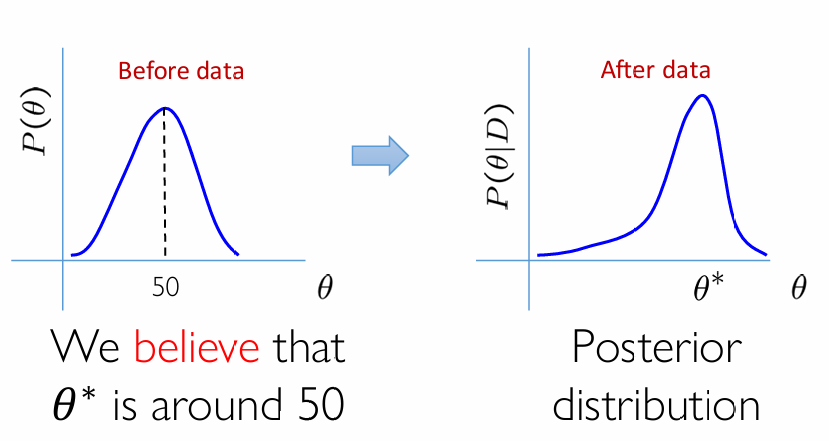
\includegraphics[width=0.72\textwidth]{./assets/Prior and Posterior Distribution.png}
        \caption{Prior and Posterior Distribution}
        \end{figure}

        下一个问题是，如何定量地描述所谓的“修正”，描述后验分布呢？贝叶斯公式（Bayes Rule）解答了这一问题：
        $$\prob (\bm{\theta} \vert \mathcal{D}) = \frac{\prob (\mathcal{D} \vert \bm{\theta}) \prob (\bm{\theta})}{\prob (\mathcal{D})}$$

        不难看出，贝叶斯公式实质上是条件概率公式的直接推论，其中$\prob (\bm{\theta} \vert \mathcal{D})$为后验分布，$\prob (\bm{\theta})$为先验分布，
        $\prob (\mathcal{D})$为观测到数据$\mathcal{D}$的概率，在采样稳定时可以视为常数。
        称$\prob (\mathcal{D} \vert \bm{\theta})$为\textbf{似然（Likelihood）}。
        显然，在求出似然后，应用贝叶斯公式即可得到后验分布。

        似然描述了在当前模型下（即参数为$\bm{\theta}$的概率模型），观察到数据$\mathcal{D}$的概率。
        在一个极端情况中，试想我们的模型已经完全描述了数据的概率分布，在观察到足够多的均匀采样数据时，似然应恰好等于$1$。
        这意味着先验分布等于后验分布，我们已不必继续修正模型。

        在实际应用时，为避免数值溢出，常使用对数似然$\log \prob (\mathcal{D} \vert \bm{\theta})$进行计算。
        另外，通常在计算时忽略$\prob (\mathcal{D})$，而是对似然和先验分布的乘积作归一化求得后验分布。

    \subsection{Understanding}

        在现代的基于贝叶斯方法的推理框架中，我们会主观制定先验概率来表达某些特定的条件，然后对观测数据的分布特征进行细致的建模，
        同时分析模型假设中的不确定性，最后制定出一组最优的决策，或者得到一个所谓的效用函数。

        贝叶斯方法有一些显著的优点：
        \begin{enumerate}
        \item 能够利用先验知识：贝叶斯方法允许在分析中结合已有的知识或条件，这对于小样本问题或不确定环境特别有用。
        \item 动态更新：随着新数据的出现，贝叶斯方法可以不断地更新概率估计。
        \item 灵活性：贝叶斯方法并不依赖于数据的特定分布，可以应用于各种复杂问题，如概率图问题。
        \end{enumerate}

        \textbf{贝叶斯方法的核心思想是不断地根据新数据更新现有的概率估计。}
        这一想法十分朴素和自然，与人类最普遍的认知方式相符合。
        因此，许多人认为贝叶斯方法是最简单，最有效，最合理的统计方法。
        同时，批评者们则着眼于贝叶斯方法所采用的频率主义之逻辑问题，亦常常对先验概率的主观性提出质疑。

        我们对上述争论不感兴趣，不置可否。
        但是，我们认为这句话应为一件事实：如果想在不确定性面前做出一致且合理的决定，那么贝叶斯方法即是最好的方法。

    \section{Bootstrap Sample}

    \subsection{Definition}

        \textbf{自助采样（Bootstrap Sample）}是一种经典的采样方法。
        在自助采样中，我们从原始数据集中有放回地随机抽取样本，重复该过程直到创建出多个新的数据集，每个新数据集的大小均与原始数据集相同。

        \begin{figure}[htbp]
        \centering
        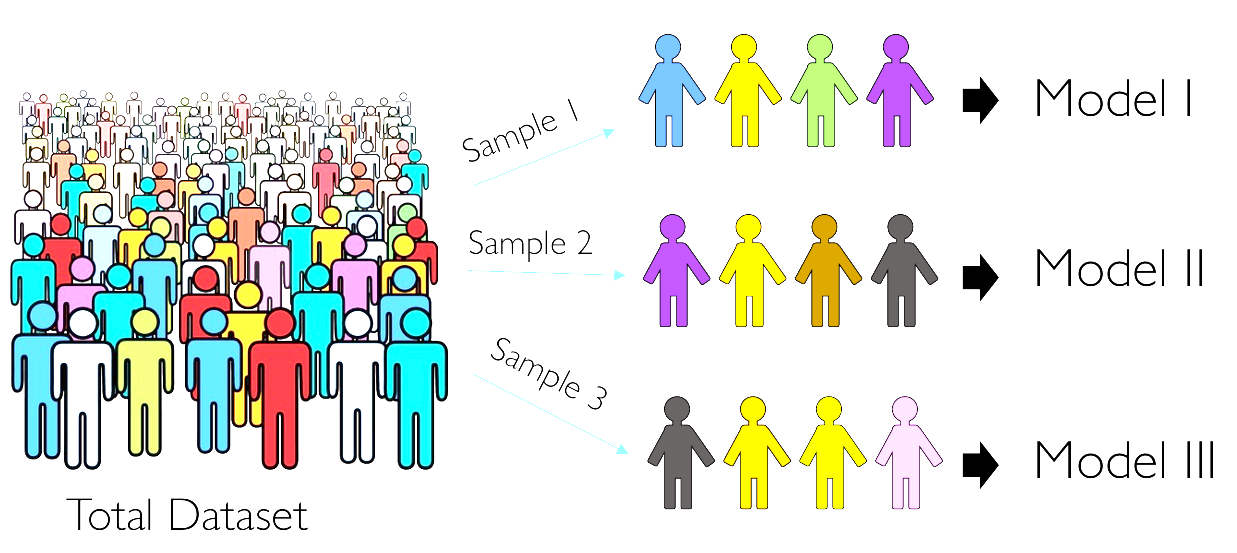
\includegraphics[width=0.90\textwidth]{./assets/Bootstrap Sample.png}
        \caption{Bootstrap Sample}
        \end{figure}

    \subsection{Mathematical Description}

        原始数据集为$\mathcal{D}_n = \{X_1, X_2, ..., X_n\}$。
        进行一次自助采样，得到数据集$\mathcal{M}_n = \{X_{t_1}, X_{t_2}, ..., X_{t_n}\}$，
        其中$\prob ({t_i} = j) = \frac{1}{n}$，$i = 1, ..., n$，$j = 1, ..., n$。

        注意到，某一样本可能在$\mathcal{M}_n$中出现多次，也可能不会出现。
        具体而言，对于任一样本$X_i$，$\prob (X_i \notin M_n) = (1 - \frac{1}{n})^n$。
        在$n$充分大时，这一概率约等于$e^{-1} = 0.368$。
        因此，我们期望有$63.2\%$的样本出现在自助采样的结果中。

    \subsection{Understanding}

        自助采样是一种非参数Monte Carlo方法，实质是对数据的重采样，进而对对总体的分布特性进行统计推断的一种方法。
        在执行自助采样时，我们可以对每个采样结果计算所需的统计量（如均值、中位数、标准差等），并据此估计原数据集的统计量及相应的置信区间。

        自助采样的优点有：
        \begin{enumerate}
        \item 无分布假设：自助采样不依赖于原始数据的分布假设，适用于非正态分布数据。
        \item 鲁棒性：通过重抽样，自助采样可以在某种意义上扩增数据，这使其在小样本情况下仍然能够表现出良好的估计性能。
        \item 随机性：自助采样得到的诸数据集间随机性较大，适合作为随机森林等集合模型的输入。
        \end{enumerate}

\end{document}
